\documentclass[tikz,border=12pt]{standalone}
\usepackage[T1]{fontenc}
\usepackage{mathpazo}
\usepackage{amsmath,amssymb}
\usetikzlibrary{arrows.meta, positioning, calc, fit, decorations.pathreplacing}

\definecolor{stblue}{HTML}{7B97AD}
\definecolor{rwgold}{HTML}{B8995E}
\definecolor{sage}{HTML}{7A9A7E}
\definecolor{dkbrown}{HTML}{3D3530}
\definecolor{wmgray}{HTML}{7B7067}
\definecolor{cream}{HTML}{F9F6F0}
\definecolor{border}{HTML}{D4C9B8}
\definecolor{terracotta}{HTML}{C47A6A}
\definecolor{lavender}{HTML}{907EA0}

\begin{document}
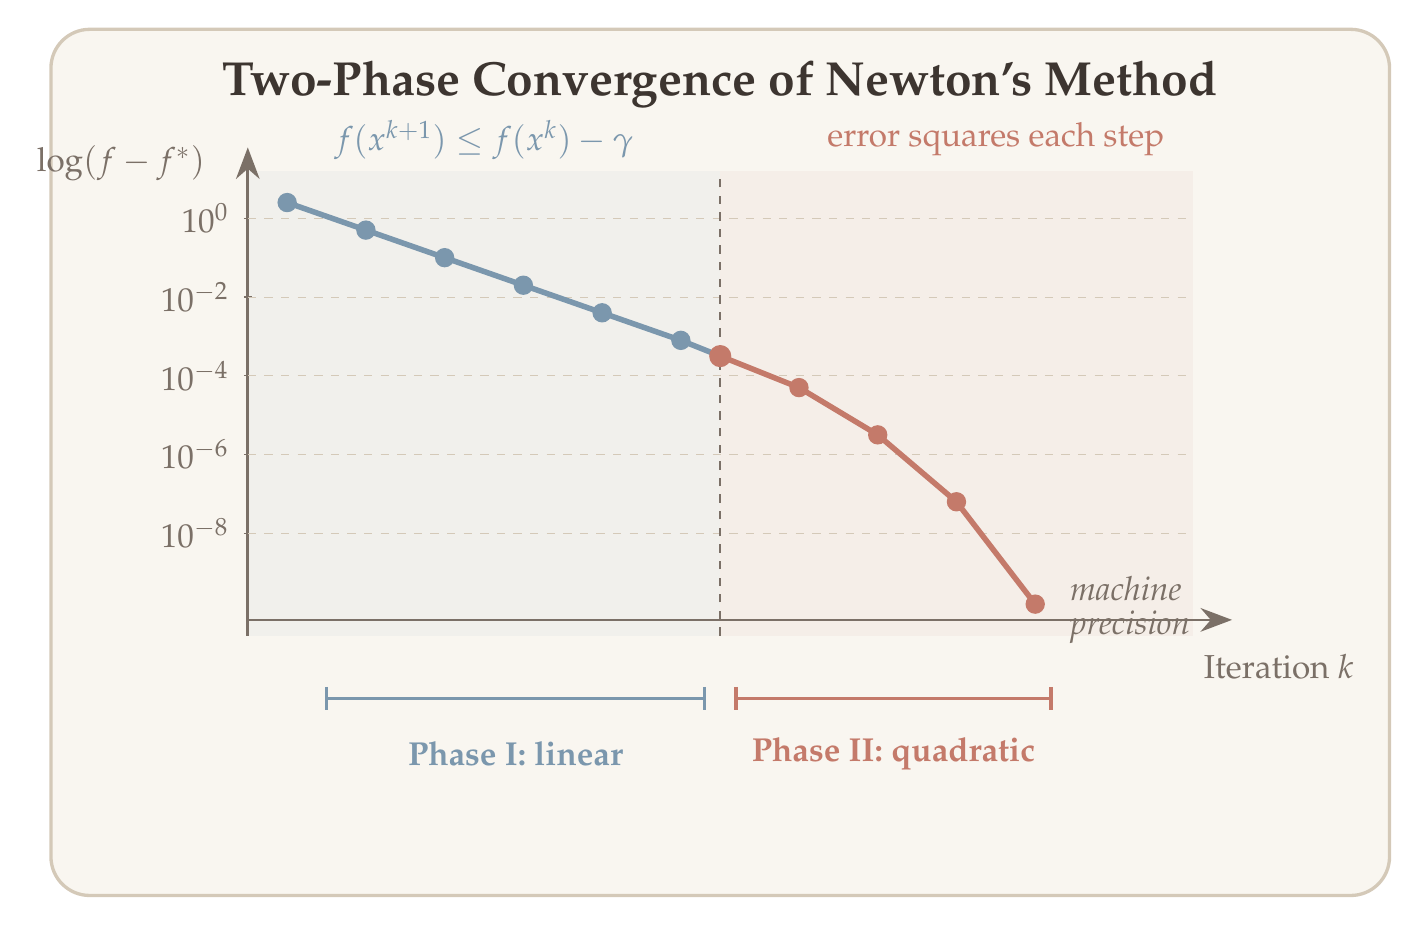
\begin{tikzpicture}[>={Stealth[length=4mm, width=3mm]}, line width=1.5pt]

% Background
\fill[cream, rounded corners=14pt] (-1.5,-3.0) rectangle (15.5,8.0);
\draw[border, line width=1.2pt, rounded corners=14pt] (-1.5,-3.0) rectangle (15.5,8.0);

% Title
\node[text=dkbrown, font=\LARGE\bfseries] at (7.0,7.3) {Two-Phase Convergence of Newton's Method};

% Phase background regions
\fill[stblue, opacity=0.06] (1.0,0.3) rectangle (7.0,6.2);
\fill[terracotta, opacity=0.06] (7.0,0.3) rectangle (13.0,6.2);

% Axes
\draw[wmgray, ->, line width=1pt] (1.0,0.5) -- (13.5,0.5);
\draw[wmgray, ->, line width=1pt] (1.0,0.3) -- (1.0,6.5);
\node[text=wmgray, font=\large, anchor=west] at (13.0,-0.1) {Iteration $k$};
\node[text=wmgray, font=\large, anchor=east] at (0.6,6.3) {$\log(f - f^*)$};

% Y-axis tick labels
\node[text=wmgray, font=\large, anchor=east] at (0.9,5.6) {$10^0$};
\draw[wmgray, line width=0.4pt] (0.95,5.6) -- (1.05,5.6);
\node[text=wmgray, font=\large, anchor=east] at (0.9,4.6) {$10^{-2}$};
\draw[wmgray, line width=0.4pt] (0.95,4.6) -- (1.05,4.6);
\node[text=wmgray, font=\large, anchor=east] at (0.9,3.6) {$10^{-4}$};
\draw[wmgray, line width=0.4pt] (0.95,3.6) -- (1.05,3.6);
\node[text=wmgray, font=\large, anchor=east] at (0.9,2.6) {$10^{-6}$};
\draw[wmgray, line width=0.4pt] (0.95,2.6) -- (1.05,2.6);
\node[text=wmgray, font=\large, anchor=east] at (0.9,1.6) {$10^{-8}$};
\draw[wmgray, line width=0.4pt] (0.95,1.6) -- (1.05,1.6);

% Grid lines
\foreach \y in {1.6,2.6,3.6,4.6,5.6} {
  \draw[border, line width=0.3pt, dashed] (1.0,\y) -- (13.0,\y);
}

% Phase I: Linear convergence
\draw[stblue, line width=2pt]
  (1.5,5.8) -- (2.5,5.45) -- (3.5,5.1) -- (4.5,4.75) -- (5.5,4.4) -- (6.5,4.05) -- (7.0,3.85);
\foreach \x/\y in {1.5/5.8, 2.5/5.45, 3.5/5.1, 4.5/4.75, 5.5/4.4, 6.5/4.05, 7.0/3.85} {
  \fill[stblue] (\x,\y) circle (3.5pt);
}

% Phase transition line
\draw[wmgray, line width=0.8pt, dashed] (7.0,0.3) -- (7.0,6.2);

% Phase II: Quadratic convergence
\draw[terracotta, line width=2pt]
  (7.0,3.85) -- (8.0,3.45) -- (9.0,2.85) -- (10.0,2.0) -- (11.0,0.7);
\fill[terracotta] (7.0,3.85) circle (4pt);
\foreach \x/\y in {8.0/3.45, 9.0/2.85, 10.0/2.0, 11.0/0.7} {
  \fill[terracotta] (\x,\y) circle (3.5pt);
}

% Phase I bracket and label
\draw[stblue, line width=1.2pt] (2.0,-0.5) -- (6.8,-0.5);
\draw[stblue, line width=1.2pt] (2.0,-0.35) -- (2.0,-0.65);
\draw[stblue, line width=1.2pt] (6.8,-0.35) -- (6.8,-0.65);
\node[text=stblue, font=\large\bfseries] at (4.4,-1.2) {Phase I: linear};
\node[text=stblue, font=\large] at (4.0,6.6) {$f(x^{k+1}) \leq f(x^k) - \gamma$};

% Phase II bracket and label
\draw[terracotta, line width=1.2pt] (7.2,-0.5) -- (11.2,-0.5);
\draw[terracotta, line width=1.2pt] (7.2,-0.35) -- (7.2,-0.65);
\draw[terracotta, line width=1.2pt] (11.2,-0.35) -- (11.2,-0.65);
\node[text=terracotta, font=\large\bfseries] at (9.2,-1.2) {Phase II: quadratic};
\node[text=terracotta, font=\large] at (10.5,6.6) {error squares each step};

% Machine precision annotation
\node[text=wmgray, font=\large\itshape, anchor=west] at (11.3,0.9) {machine};
\node[text=wmgray, font=\large\itshape, anchor=west] at (11.3,0.4) {precision};

\end{tikzpicture}
\end{document}
